\section{Diccionario de datos}

  \paragraph{}Para concluir el análisis funcional, se especificará la
  transformación que los elementos sufren en el interior del sistema, así como
  todas las relaciones existentes entre ellos. Esto se realizará mediante otra
  técnica de descripción muy extendida como es el \textit{Diccionario de datos}
  (DD).

  \paragraph{}El Diccionario de datos es una lista organizada de los datos
  utilizados en el sistema y que gráficamente se encuentran presentes en los
  flujos de datos y en los almacenes del conjunto de los diagramas de flujo de
  datos. Esta técnica es utilizada para representar a cualquier dato elemental,
  independientemente de su complejidad, que ha sido o no considerado en la
  moderación de la información mediante las técnicas correspondientes. Su
  función es la especificación de cualquier elemento de información que es
  manejado por una función, definiéndose claramente de esta forma la interfaz
  de la misma.

  \paragraph{}El Diccionario de datos va a estar estructurado de la siguiente
  manera:

  \begin{description}
   \item[Nombre] Denominación del elemento de datos o de control, de la
                 base de datos, o de la entidad externa.
   \item[Alias]  Otras denominaciones utilizadas para la misma entrada.
   \item[Uso]    Relación de procesos que hacen uso del elemento de datos o de
                 control.
   \item[Descripción] Contenido de lo representado mediante una notación.
   \item[Información adicional] Otras anotaciones de interés.
  \end{description}

\subsection{Entidades externas}

  \subsubsection{Teclado}

  \paragraph{}prueba.

\subsection{Almacenes de datos}

  \subsubsection{Base de datos}

  \begin{center}
  \begin{tabular}{| l | p{9cm} |}
    \hline
    Nombre & \textbf{Base de datos}.\\
    \hline
    Alias & Ninguno.\\
    \hline
    \multirow{5}{*}{Uso} & Entrada/salida de los siguientes procesos:\\
                         & - Proceso 2 (Módulo Administrador principal).\\
                         & - Proceso 3 (Módulo Administrador de centro).\\
                         & - Proceso 4 (Módulo Asesores).\\
                         & - Proceso 5 (Módulo Alumnos).\\
    \hline
    Descripción & Sistema software donde se almacenan los datos de la
                  aplicación.\\
    \hline
    Información adicional & Ninguna.\\
    \hline
  \end{tabular}
\end{center}


  \subsubsection{Copia de seguridad}

  \paragraph{}El usuario administrador principal puede realizar copias de
seguridad de la información existente en la aplicación o restaurar una copia
anteriormente realizada.

\paragraph{}La figura \ref{diagramaNivel3-CopiaSeguridad}
muestra el nivel de abstracción 3: Copia de seguridad.

  \begin{figure}[!ht]
    \begin{center}
      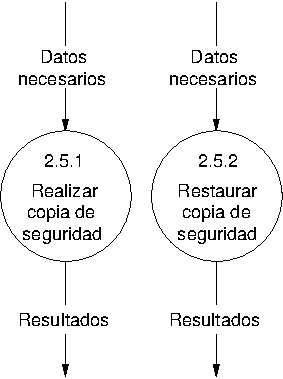
\includegraphics[]{08.Analisis_Funcional/8.2.DFDs/Niveles/Nivel3/AdministradorPrincipal/CopiaSeguridad/Diagramas/nivel3-CopiaSeguridad.pdf}
      \caption{Nivel de abstracción 3: Copia de seguridad.}
      \label{diagramaNivel3-CopiaSeguridad}
    \end{center}
  \end{figure}


\subsection{Elementos de información}

  \subsubsection{Datos teclado}

  \begin{center}
  \begin{tabular}{| l | p{9cm} |}
    \hline
    Nombre & \textbf{Datos teclado}.\\
    \hline
    Alias & Ninguno.\\
    \hline
    \multirow{3}{*}{Uso} & Entrada de los siguientes procesos:\\
                         & - Proceso 0 (Asesorías Académicas).\\
                         & - Proceso 1 (Procesar entrada).\\
    \hline
    Descripción & Representa todos los datos y órdenes introducidas en la
                  aplicación por el usuario mediante el teclado.\\
    \hline
    Información adicional & Ninguna.\\
    \hline
  \end{tabular}
\end{center}


  \subsubsection{Datos ratón}

  \begin{center}
  \begin{tabular}{| l | p{9cm} |}
    \hline
    Nombre & \textbf{Datos ratón}.\\
    \hline
    Alias & Ninguno.\\
    \hline
    \multirow{5}{*}{Uso} & Entrada de los siguientes procesos:\\
                         & - Proceso 0 (Asesorías Académicas).\\
                         & - Proceso 1 (Procesar entrada).\\
                         & Salida de la siguiente entidad:\\
                         & - Ratón.\\
    \hline
    Descripción & Representa todos los datos y órdenes introducidas en la
                  aplicación por el usuario mediante el teclado.\\
    \hline
    Información adicional & Ninguna.\\
    \hline
  \end{tabular}
\end{center}


  \subsubsection{Fecha del sistema}

  \begin{center}
  \begin{tabular}{| l | p{9cm} |}
    \hline
    Nombre & \textbf{Fecha del sistema}.\\
    \hline
    Alias & Ninguno.\\
    \hline
    \multirow{5}{*}{Uso} & Entrada de los siguientes procesos:\\
                         & - Proceso 0 (Asesorías Académicas).\\
                         & - Proceso 1 (Procesar entrada).\\
                         & Salida de la siguiente entidad:\\
                         & - Sistema.\\
    \hline
    Descripción & Representa la fecha y hora del sistema en el que estará
                  alojada la aplicación.\\
    \hline
    Información adicional & Ninguna.\\
    \hline
  \end{tabular}
\end{center}


  \subsubsection{Datos recuperados}

  \begin{center}
  \begin{tabular}{| l | p{9cm} |}
    \hline
    Nombre & \textbf{Datos recuperados}.\\
    \hline
    Alias & Ninguno.\\
    \hline
    \multirow{6}{*}{Uso} & Entrada de los siguientes procesos:\\
                         & - Proceso 0 (Asesorías Académicas).\\
                         & - Proceso 2 (Administrador principal).\\
                         & - Proceso 2.1 (Validar administrador).\\
                         & Salida del siguiente almacén:\\
                         & - Copia de seguridad.\\
    \hline
    Descripción & Representa los datos recuperados de una copia de seguridad.
\\
    \hline
    Información adicional & Ninguna.\\
    \hline
  \end{tabular}
\end{center}


  \subsubsection{Datos almacenados}

  \begin{center}
  \begin{tabular}{| l | p{9cm} |}
    \hline
    Nombre & \textbf{Datos almacenados}.\\
    \hline
    Alias & Ninguno.\\
    \hline
    \multirow{5}{*}{Uso} & Entrada del siguiente almacén:\\
                         & - Copia de seguridad.\\
                         & Salida de los siguientes procesos:\\
                         & - Proceso 0 (Asesorías Académicas).\\
                         & - Proceso 2 (Administrador principal).\\
                         & - Proceso 2.7 (Procesar salida).\\
    \hline
    Descripción & Representa los datos comprimidos tras realizar una copia de
                  seguridad.\\
    \hline
    Información adicional & Ninguna.\\
    \hline
  \end{tabular}
\end{center}


  \subsubsection{Información consultada}

  \begin{center}
  \begin{tabular}{| l | p{9cm} |}
    \hline
    Nombre & \textbf{Información consultada}.\\
    \hline
    Alias & Ninguno.\\
    \hline
    \multirow{5}{*}{Uso} & Entrada de la siguiente entidad:\\
                         & - Pantalla.\\
                         & Salida de los siguientes procesos:\\
                         & - Proceso 0 (Asesorías Académicas).\\
                         & - Proceso 2 (Administrador principal).\\
                         & - Proceso 3 (Administrador de centro).\\
                         & - Proceso 4 (Asesores).\\
                         & - Proceso 5 (Alumnos).\\
                         & - Procesos 2.7, 3.6, 4.6 y 5.6 (Procesar salida).\\
    \hline
    Descripción & Representa la información que será proporcionada por la
                  aplicación y que será visualizada por pantalla.\\
    \hline
    Información adicional & Ninguna.\\
    \hline
  \end{tabular}
\end{center}


  \subsubsection{Resultados de operaciones}

  \begin{center}
  \begin{tabular}{| l | p{9cm} |}
    \hline
    Nombre & \textbf{Resultados de operaciones}.\\
    \hline
    Alias & Ninguno.\\
    \hline
    \multirow{9}{*}{Uso} & Entrada de la siguiente entidad:\\
                         & - Pantalla.\\
                         & Salida de los siguientes procesos:\\
                         & - Proceso 0 (Asesorías Académicas).\\
                         & - Proceso 2 (Administrador principal).\\
                         & - Proceso 3 (Administrador de centro).\\
                         & - Proceso 4 (Asesores).\\
                         & - Proceso 5 (Alumnos).\\
                         & - Procesos 2.7, 3.6, 4.6 y 5.6 (Procesar salida).\\
    \hline
    Descripción & Resultados obtenidos a partir de las diferentes operaciones
                  realizadas a los datos manipulados por la aplicación.\\
    \hline
    Información adicional & Ninguna.\\
    \hline
  \end{tabular}
\end{center}


  \subsubsection{Mensajes de error}

  \begin{center}
  \begin{tabular}{| l | p{9cm} |}
    \hline
    Nombre & \textbf{Mensajes de error}.\\
    \hline
    Alias & Ninguno.\\
    \hline
    \multirow{5}{*}{Uso} & Entrada de la siguiente entidad:\\
                         & - Pantalla.\\
                         & Salida de los siguientes procesos:\\
                         & - Proceso 0 (Asesorías Académicas).\\
                         & - Proceso 2 (Administrador principal).\\
                         & - Proceso 3 (Administrador de centro).\\
                         & - Proceso 4 (Asesores).\\
                         & - Proceso 5 (Alumnos).\\
                         & - Procesos 2.7, 3.6, 4.6 y 5.6 (Procesar salida).\\
    \hline
    Descripción & Mensajes de error obtenidos durante la manipulación del
                  sistema.\\
    \hline
    Información adicional & Ninguna.\\
    \hline
  \end{tabular}
\end{center}


  \subsubsection{Información impresa}

  \begin{center}
  \begin{tabular}{| l | p{9cm} |}
    \hline
    Nombre & \textbf{Información impresa}.\\
    \hline
    Alias & Ninguno.\\
    \hline
    \multirow{9}{*}{Uso} & Entrada de la siguiente entidad:\\
                         & - Impresora.\\
                         & Salida de los siguientes procesos:\\
                         & - Proceso 0 (Asesorías Académicas).\\
                         & - Proceso 2 (Administrador principal).\\
                         & - Proceso 3 (Administrador de centro).\\
                         & - Proceso 4 (Asesores).\\
                         & - Proceso 5 (Alumnos).\\
                         & - Procesos 2.7, 3.6, 4.6 y 5.6 (Procesar salida).\\
    \hline
    Descripción & Mensajes de error obtenidos durante la manipulación del
                  sistema.\\
    \hline
    Información adicional & Ninguna.\\
    \hline
  \end{tabular}
\end{center}

